
%----------------------------------------------------------------------------------------
%	CHAP Functions
%----------------------------------------------------------------------------------------

\chapterimage{blue-chapter-head_4-reduced.pdf} % Chapter heading image

\chapter{R Functions}\label{chap:RFunctions}\index{Functions}\index{R Functions}

\section{Overview}
Since version 1.4, MetaR supports calling R functions directly. This Chapter describes how you can use this feature to take advantage of the many functions available in R packages to transform data in your MetaR Analyses. 

\section{Function Stubs}
Function stubs\index{Function stubs} are provided that represent functions offered by different packages. Stubs do not provide the code associated with the function, but describe the function name and the arguments of the function and its default values. This information is used to support auto-completion for R functions. 

We provide pre-imported stubs for the packages used during the MetaR training sessions, namely: \textit{base}, \textit{graphics}, \textit{data.table}, \textit{pheatmap}, \textit{biomaRt}, \textit{edgeR} and \textit{limma}. While stubs are provided, they are not immediately available in a MetaR analysis. In order to use R function stubs, you need to 
\begin{itemize}
  \item Add \textit{org.campagnelab.R} to the list of Used languages in the model where you need the stubs.
  \item Use the \texttt{import stubs} statement followed with the name of the package that provides the functions that you wish to use.
\end{itemize}

\noindent{}For instance, if you enter the following statement: 
\begin{lstlisting}
import stubs base
\end{lstlisting}

\noindent{}After typing this statement, the \textit{base} package R functions will become available inside the Analysis where you imported these stubs. You can use R function using the \texttt{eval} statement or expression (see Sections~\ref{sec:EvalStatement}and \ref{sec:EvalExpression}).

If you need a package that is not yet provided with MetaR, you should use the \texttt{import package} statement (see Section~\ref{sec:ImportPackageStatement}). 

\section{Import Stubs Statement}\label{sec:ImportStubsStatement}\index{Import function stubs}
The \texttt{import stubs} statement (alias import stubs) makes it possible to import functions in packaged already packaged with MetaR. Simply type import stubs, and use auto-completion to locate the package for which you need to import function stubs.


\section{Import Package Statement}\label{sec:ImportPackageStatement}\index{Import package}

The \texttt{import package} statement (alias import package) makes it possible to import functions in any R package. If the package is already provided in MetaR, the \texttt{import package} statement  will be automatically replaced with the equivalent \texttt{import stubs} statement (see Section~\ref{sec:ImportStubsStatement}). Figure~\ref{fig:NewImportPackage} presents an import package statement. 
\paragraph{name} The name attribute is a string and must be the name of an R package, suitable to install the package in R with  \texttt{install.packages("name")}.

\begin{figure}[h!tbp]
  \centering
  
\includegraphics[width=\figWidthSmall]{figures/NewImportPackage.pdf}
\caption[New Import Package Statement.]{\textbf{New Import Package Statement.}  Enter the name of an R package to import this package into the Analysis. Note that the package will be visible only after you run the Analysis at least once.}
\label{fig:NewImportPackage}
\end{figure}

\begin{remark}
If you need to import a Bioconductor package, use the \texttt{import bioconductor package} statement instead.
\end{remark}
After you execute the Analysis that contains the import package statement, the package will be installed in the version of R that you are using, if needed and the package loaded. 
Use the ``Reload Functions and Create Stubs'' intention after you have executed the statement to create the Stubs root node for the functions in the package. When you call this intention, the package will be inspected for function declarations, and these declarations will be written to a \texttt{Stubs} root node in the model where the \texttt{Analysis} is located. Following this process, the \texttt{import package} statement is replaced with the import stubs statement, loading the stubs directly from the model. Note that you can inspect the stubs object to learn about the functions available in the package represented by the stubs. 


\section{Import Bioconductor Package Statement}\label{sec:ImportBioconductorPackageStatement}\index{Import bioconductor package}\index{Bioconductor}
Importing a bioconductor package is very similar to importing a regular R package, but you need to use the \texttt{import bioconductor package} statement. This statement ensure appropriate installation and loading of bioconductor packages in R. Figure~\ref{fig:NewBioconductorImportPackage} presents a new \texttt{import bioconductor package} statement.

\begin{figure}[h!tbp]
  \centering
  
\includegraphics[width=\figWidthNarrow]{figures/NewImportBioconductorPackage.pdf}
\caption[New Import Bioconductor Package Statement.]{\textbf{New Bioconductor Import Package Statement.}  Enter the name of an Bioconductor package to import this package into the Analysis. Note that the package will be visible only after you run the Analysis at least once.}
\label{fig:NewBioconductorImportPackage}
\end{figure}

\section{Stubs}\index{Stubs}
Stubs represent functions from R regular or bioconductor packages. We do not recommend creating Stubs manually. The easiest way to create Stub root nodes is by using the \texttt{import package} and \texttt{import bioconductor package} statements. Figure~\ref{fig:StubsExample} presents a snapshot showing a few functions located in the base Stubs root node (R version 3.1.3).
\begin{remark}
Stubs distributed with MetaR are packaged in models named after the version of R which provided the package, in an effort to help track differences between major R versions.
\end{remark}


\begin{figure}[h!tbp]
  \centering
  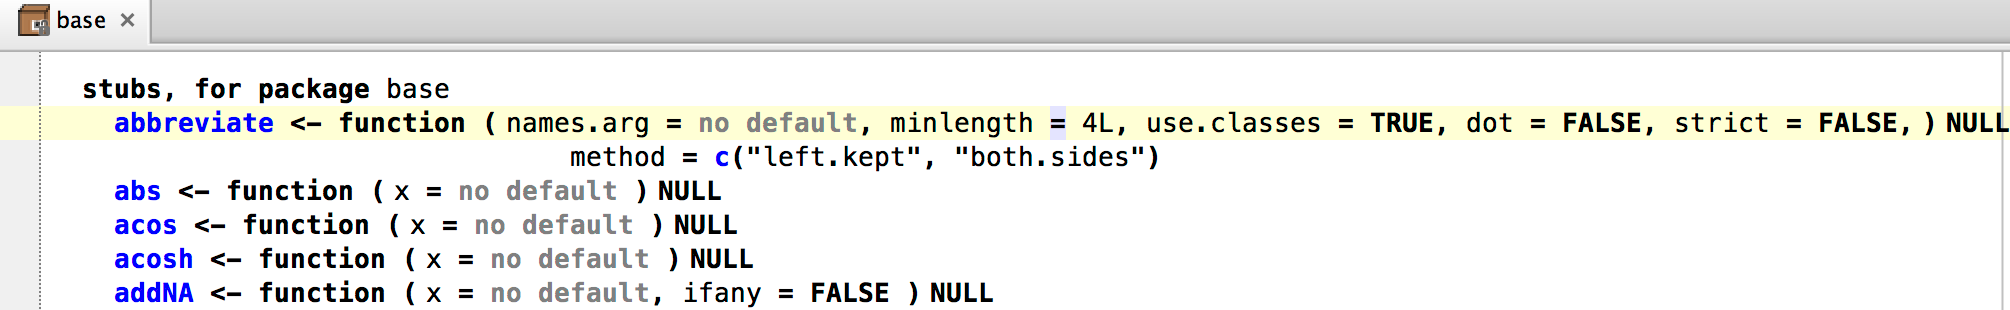
\includegraphics[width=\figWidthWide]{figures/BaseStubsSnapshot.png}
\caption[Base Package Stubs Illustration.]{\textbf{Base Package Stubs Illustration.}  This snapshot presents the beginning of the stubs base root node, located in model \texttt{R3\_1\_3} (language \textit{org\allowbreak{}.campagnelab\allowbreak{}.metar\allowbreak{}.r\allowbreak{}.stubs}).}
\label{fig:StubsExample}
\end{figure}

\section{Eval Statement}\label{sec:EvalStatement}
The \texttt{eval} statement can be used to call R functions that produce some side-effect. When you import the devkit \textit{org.campagnelab.R} into a model, you can type \texttt{eval} in an Analysis node as a statement. The statement will offer auto-completion for function names imported into the analysis. If you do not see the function that you would like to use, make sure you have imported the stubs for the package that contains this function. When you run the analysis, the function named after \texttt{eval} will be executed. Note that you cannot retrieve a return value with the \texttt{eval} statement. You must use the \texttt{eval} expression to obtain a value. The eval statement is useful when you need to call a function that has a side-effect, for instance the setkey function of data.table.

\section{Eval Expression}\label{sec:EvalExpression}
The \texttt{eval} expression can be used to call R functions inside a MetaR expression. MetaR expressions are used in the \texttt{subset} statement, and in some plotting statements (e.g., \texttt{boxplot} or \texttt{histogram}).  When you import the devkit \textit{org.campagnelab.R} into a model, you can type \texttt{eval} inside an expression. The \texttt{eval} expression will offer auto-completion for function names imported into the analysis. If you do not see the function that you would like to use, make sure you have imported the stubs for the package that contains this function. 


\section{Accessing MetaR Columns within R Expressions}\label{sec:AccessingMetaRColumns}\index{Accessing MetaR columns within R expressions}
When you use either the eval statement or expression, you will often need to access columns from a MetaR table to pass as arguments to the function. You can do this with the \texttt{\$} node, which bridges between R expressions (used inside R functions) and MetaR columns. After typing \texttt{\$}, the node will auto-complete to the set of columns visible at this point of the MetaR \texttt{Analysis}. 


\section{Example}
Figure~\ref{fig:TestinFunctionsExample} presents an example where stubs are imported for packages pre-packaged with MetaR and the import package statement is used to import grDevices.
\begin{figure}[h!tbp]
  \centering
  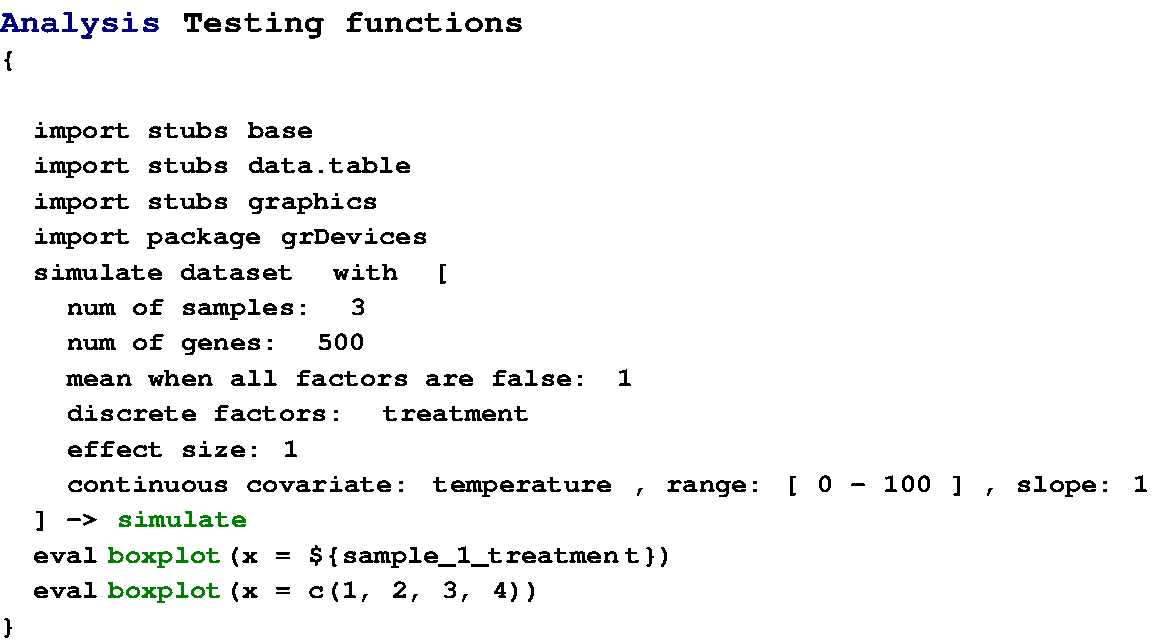
\includegraphics[width=\figWidthWide]{figures/TestinFunctionsExample.pdf}
\caption[Functions Example.]{\textbf{Functions Example.} This example imports stubs and one package, creates a table with three columns (see Simulate statement in Chapter~\ref{chap:SimulatingDatasets}) and evaluates two R functions. The first use of the \texttt{boxplot} function plots the values of the column \texttt{sample\_1\_treatment} that was generated with the simulate statement. The second call to \texttt{boxplot} is given a list of four integers.}
\label{fig:TestinFunctionsExample}
\end{figure}

